\documentclass[11pt,a4paper]{article}

\usepackage[utf8]{inputenc}
\usepackage[T1]{fontenc}
\usepackage{lmodern}
\usepackage[margin=2.5cm]{geometry}
\usepackage{microtype}
\usepackage{graphicx}
\usepackage{booktabs}
\usepackage{tabularx}
\usepackage{array}
\usepackage{xcolor}
\usepackage{enumitem}
\usepackage{caption}
\usepackage[section]{placeins}   % keep floats inside their own section
\usepackage{fancyhdr}
\usepackage{titlesec}
\usepackage[colorlinks=true,linkcolor=blue!50!black,urlcolor=blue!50!black,citecolor=blue!50!black]{hyperref}
\hypersetup{pdftitle={NUMAlloc Evaluation on CXL-Enabled Hardware},pdfauthor={Adam Bekkar},
  pdfsubject={Evaluation of NUMAlloc, a NUMA-aware memory allocator, on a server with CXL memory, and the design of a CXL-aware allocator.},
  pdfkeywords={memory allocation, NUMA, CXL, hugepages, TLB, NUMAlloc}}

\setlength{\parskip}{0.6em}
\setlength{\parindent}{0pt}
\setlength{\emergencystretch}{2em}
\linespread{1.08}

% Section headings
\titleformat{\section}{\Large\bfseries\sffamily}{\thesection}{0.7em}{}
\titleformat{\subsection}{\large\bfseries\sffamily}{\thesubsection}{0.7em}{}
\titlespacing*{\section}{0pt}{2.2ex plus 0.5ex}{1.2ex}
\titlespacing*{\subsection}{0pt}{1.8ex plus 0.4ex}{0.8ex}

% Captions
\captionsetup{font=small,labelfont={bf,sf},format=hang,justification=raggedright,singlelinecheck=false,skip=6pt}

% Header / footer
\pagestyle{fancy}
\fancyhf{}
\renewcommand{\headrulewidth}{0.3pt}
\fancyhead[L]{\small\sffamily NUMAlloc Evaluation on CXL-Enabled Hardware}
\fancyhead[R]{\small\sffamily Adam Bekkar}
\fancyfoot[C]{\small\thepage}
\setlength{\headheight}{14pt}

% Better float placement
\renewcommand{\topfraction}{0.9}
\renewcommand{\bottomfraction}{0.8}
\renewcommand{\textfraction}{0.1}
\renewcommand{\floatpagefraction}{0.7}

% Images are looked up in ./images/ first, then in the current directory.
\graphicspath{{images/}{./}}

% Figure helpers. Usage: \fig{file}{width}{caption}, \figtwo{f1}{f2}{caption}, \figthree{f1}{f2}{f3}{caption}
% A figure whose image file is missing is left out.
\newcommand{\fig}[3]{\IfFileExists{images/#1}{\figreal{#1}{#2}{#3}}{}}
\newcommand{\figreal}[3]{%
  \begin{figure}[!htbp]
    \centering
    \includegraphics[width=#2\textwidth,height=0.7\textheight,keepaspectratio]{#1}
    \caption{#3}
  \end{figure}}

\newcommand{\opt}[1]{\texttt{#1}}

\newcommand{\figtwo}[3]{\IfFileExists{images/#1}{\figtworeal{#1}{#2}{#3}}{}}
\newcommand{\figtworeal}[3]{%
  \begin{figure}[!htbp]
    \centering
    \begin{minipage}[t]{0.485\textwidth}\centering
      \includegraphics[width=\linewidth,height=0.4\textheight,keepaspectratio]{#1}
    \end{minipage}\hfill
    \begin{minipage}[t]{0.485\textwidth}\centering
      \includegraphics[width=\linewidth,height=0.4\textheight,keepaspectratio]{#2}
    \end{minipage}
    \caption{#3}
  \end{figure}}

\newcommand{\figthree}[4]{\IfFileExists{images/#1}{\figthreereal{#1}{#2}{#3}{#4}}{}}
\newcommand{\figthreereal}[4]{%
  \begin{figure}[!htbp]
    \centering
    \begin{minipage}[t]{0.32\textwidth}\centering
      \includegraphics[width=\linewidth,height=0.35\textheight,keepaspectratio]{#1}
    \end{minipage}\hfill
    \begin{minipage}[t]{0.32\textwidth}\centering
      \includegraphics[width=\linewidth,height=0.35\textheight,keepaspectratio]{#2}
    \end{minipage}\hfill
    \begin{minipage}[t]{0.32\textwidth}\centering
      \includegraphics[width=\linewidth,height=0.35\textheight,keepaspectratio]{#3}
    \end{minipage}
    \caption{#4}
  \end{figure}}

\title{\sffamily\bfseries NUMAlloc Evaluation on CXL-Enabled Hardware}
\author{Adam Bekkar\\[0.4em]
\normalsize Research internship at the RS3 Lab, EPFL\\
\normalsize With Prof.\ Sanidhya Kashyap, supervised by Musa \"Unal\\
\normalsize BSc in Computer Science, EPFL\\
\normalsize MSc student in Computer Science at ETH Zurich}
\date{June to August 2026}

\begin{document}
\maketitle

%------------------------------------------------------------
\section{Project Overview}

\subsection*{Description}

This project evaluates NUMAlloc, a NUMA-aware memory allocator presented at ISMM~'23~\cite{numalloc}, on a CXL-enabled server of the lab (4~NUMA nodes: 2~CPU nodes with local DDR memory, plus 2~CXL memory nodes with no CPUs). The goals are, first, to replicate the paper's core performance comparison (its ``Figure~4: runtime, remote accesses, and TLB misses across six memory allocators''), and second, to assess whether NUMAlloc's binding-based design generalizes to CXL memory, which the original paper did not test. The scripts, the source-code fixes and the raw results are public~\cite{repo}.

\subsection*{NUMAlloc's Main Objective}

NUMA machines split memory across multiple nodes, each attached to a specific set of CPU cores. A thread can access memory on its own node quickly (a ``local'' access), but accessing memory that lives on a different node is significantly slower (a ``remote'' access); our own locality test on this machine measured a 23--28\% bandwidth penalty for this. Left to its own devices, a regular allocator has no awareness of this at all: it might hand a thread memory that happens to sit on a different node, or a thread might get migrated by the OS scheduler to a different node than where its memory actually lives. Both silently turn what should be fast local accesses into slow remote ones.

NUMAlloc's core idea is to fix this at the allocator level: it explicitly binds each thread to a specific NUMA node, and explicitly binds each region of memory to a specific node too, so it always knows exactly which node a thread is on and always gives that thread memory from its own node. This is what the paper calls \emph{binding-based memory management}, the first of its kind, since prior NUMA-aware allocators (e.g., TCMalloc-NUMA) only bind memory, not threads, so a thread migrated by the OS scheduler can end up far from its own memory without the allocator ever knowing.

Two further mechanisms build on this binding:
\begin{itemize}[nosep]
  \item \textbf{Origin-aware memory management}, where both allocations and deallocations respect an object's original node: freed objects go back to a freelist matching their origin (not just wherever the freeing thread happens to be), so memory reused later does not gradually drift to the wrong node.
  \item \textbf{Incremental sharing}, where threads on the same node share a single hugepage, each drawing only the small amount they need rather than claiming a whole 2\,MB page. This gives NUMAlloc hugepage-level TLB benefits without the memory waste a naive hugepage approach would cost.
\end{itemize}

As for why it uses ``node-interleaved'' binding by default: NUMAlloc needs some rule for deciding which node each new thread gets bound to, and the simplest option is to hand them out round-robin (thread~1 to node~0, thread~2 to node~1, thread~3 back to node~0, and so on) so that every node ends up with a similar number of threads. The paper also describes an alternative (``node-saturate'': fill up one node completely before moving to the next), which it found works better only if you are deliberately using just part of the machine's cores. Since these experiments use all available cores, node-interleaved is the right default here too.

%------------------------------------------------------------
\section{Bugs Identified and Fixed in NUMAlloc}

NUMAlloc has not been updated since approximately 2020, while the machine used for these experiments runs a much newer Linux kernel and glibc version. Several of NUMAlloc's internal mechanisms were written against assumptions about the C library and kernel that no longer hold on current systems, which produced the following issues, found and fixed in the course of building and testing NUMAlloc on the machine.

\paragraph{Thread-creation interposition failure on modern glibc.}
NUMAlloc intercepts every thread creation by defining its own \texttt{pthread\_create()} and using it in place of the real one, then looking up the real one at runtime to actually create the thread. Before glibc~2.34, that lookup reliably found the real function because it lived in a separate library. But glibc~2.34 merged pthread's code directly into glibc itself, removing that separation. The lookup therefore broke and NUMAlloc's own version ended up calling itself instead of the real function. Fixed by correcting how the real function is resolved~\cite{glibc234}.

\paragraph{Crash on large allocations (SIGBUS).}
Caused by an insufficient static hugepage reservation on the machine's compute nodes relative to NUMAlloc's memory needs. Resolved by reserving enough static hugepages; I confirmed that the same crash reproduces predictably whenever total demand exceeds the reservation, and disappears when it does not.

I checked NUMAlloc's source directly to confirm this: large allocations (above 4\,MB) explicitly request memory with the \texttt{MAP\_HUGETLB} flag (\texttt{mm.hh}), which is only satisfied from the static pool, not from THP. This is compiled into the build (the Makefile defines \texttt{USE\_HUGE\_PAGE}).

THP is still used and needed separately, for NUMAlloc's ``incremental sharing'' mechanism (Section~3.4 in the paper), which lets threads share a hugepage efficiently. So NUMAlloc relies on both: THP for its normal adaptive layout, and an explicit static reservation for large allocations specifically.

\paragraph{Thread-slot exhaustion under high thread-churn workloads.}
Fixed via a thread-local-storage destructor that properly releases a thread's slot on exit. I verified that this fix does not introduce any measurable performance cost on real benchmark workloads.

\paragraph{Missing \texttt{malloc\_usable\_size()} implementation.}
Root cause of a hard crash under MPI-based workloads (LAMMPS, Quicksilver, etc.).

The last one is worth expanding on. As NUMAlloc never implements the standard \texttt{malloc\_usable\_size()} function, any program that calls it on a NUMAlloc-managed pointer silently falls through to glibc's own implementation, which misreads NUMAlloc's internal memory layout as if it were glibc's own, corrupting memory. This was confirmed with a minimal, MPI-unrelated reproduction (a single call to \texttt{getent passwd}, which internally happens to call this function) before being traced back to explain the original MPI crash. To fix this issue, I used an external interposition library, requiring no changes to NUMAlloc's own source code; it was tested and confirmed to resolve real workload crashes.

\medskip
\noindent\textbf{Note.} LAMMPS and Quicksilver, the two MPI-based applications used to show this bug, are not part of the final Figure~4 comparison below. Getting even a single clean run required stacking three separate compatibility shims on top of NUMAlloc (working around the \texttt{malloc\_usable\_size} bug, plus two further NUMA binding issues that only surfaced once the first was fixed), and even then it only worked reliably within a single NUMA node, not at the full multi-node scale these applications are meant to run at. Given how much extra work this required for a comparison that would still be compromised, I did not pursue it further during the internship.

%------------------------------------------------------------
\section{NUMA and CXL Locality Effects Are Real on This Hardware}

Before drawing conclusions about allocator behavior, I built an allocator-independent test to confirm that memory locality actually matters on this specific machine. A single-threaded, memory-bandwidth-bound benchmark was run three times, changing nothing except where the OS was told to physically place its memory: on the local CPU node, on the other (remote) CPU node, or on a CXL memory node.

This benchmark uses a sequential access pattern: each thread walks a large buffer from start to end, reading and rewriting every element, repeated over several passes (the same way as the classic STREAM benchmark). ``Effective bandwidth'' is the resulting throughput: total bytes moved (counting both the read and the write of each element) divided by elapsed time, combined across all threads. This deliberately isolates raw memory bandwidth rather than testing allocation/deallocation behavior. Unlike the Hoard suite or PARSEC benchmarks, which stress the allocator itself, this test measures the hardware's actual memory bandwidth under different placement conditions, with the allocator playing no role at all.

\fig{numa_locality.png}{0.8}{Effective memory bandwidth for local, remote-CPU-node, and CXL placement (local: 14.9\,GB/s; CXL: 10.7\,GB/s).}

%------------------------------------------------------------
\section{Early Baseline: The Hoard Benchmark Suite and Pbzip2}

Before building the full PARSEC-based Figure~4 replication, I first ran a quicker round of experiments using the Hoard synthetic benchmark suite, a small, fast set of allocator stress tests (larson, threadtest, cache-scratch, cache-thrash), alongside Pbzip2, to get an initial sense of how NUMAlloc compares to other allocators before committing to the larger PARSEC-based comparison.

Pbzip2 compression showed no meaningful runtime difference between any of the six allocators: all finish within 0.01 seconds of each other. NUMAlloc's peak memory usage on Pbzip2 is notably lower than every competitor (74\,MB vs.\ 267--465\,MB), though I am treating that specific number cautiously rather than as a confirmed result.

\figtwo{pbzip2_comparison_performance_default.png}{pbzip2_comparison_memory_default.png}{Pbzip2 baseline across the six allocators.}

cache-scratch and cache-thrash show no meaningful difference between any allocator at any thread count. larson (a throughput test) shows NUMAlloc as the slowest of all six allocators at every thread count tested, consistent with the paper's own admission that it underperforms on this specific benchmark.

\figtwo{allocator_comparison_performance_default.png}{allocator_comparison_memory_default.png}{Hoard benchmark suite results across thread counts.}

The table below breaks this down further, showing each benchmark's actual working set, what specifically it stresses in an allocator, and the measured allocation/deallocation throughput at 96 threads.

\begin{table}[htbp]
\centering
\small
\renewcommand{\arraystretch}{1.25}
\begin{tabularx}{\textwidth}{@{}p{1.7cm} >{\raggedright\arraybackslash}p{3.7cm} >{\raggedright\arraybackslash}p{3.4cm} >{\raggedright\arraybackslash}X@{}}
\toprule
\textbf{Benchmark} & \textbf{Working set} & \textbf{Why it stresses allocators} & \textbf{Alloc+dealloc rate (ops/s) at 96 threads} \\
\midrule
larson &
8--1000 byte objects, 5000/thread, passed between threads &
Remote deallocation: objects freed by a different thread than the one that allocated them &
glibc: 1.12B, NUMAlloc: 691M, jemalloc: 1.34B, TCMalloc: 1.50B, TBB: 907M, mimalloc: 1.72B \\
\addlinespace
threadtest &
64-byte objects (8-element arrays of a 2-int struct), $\sim$1B total allocations across all threads combined, no cross-thread interaction &
Per-thread throughput with zero contention: the best case for per-thread caching allocators &
glibc: 3.86B, NUMAlloc: 3.70B, jemalloc: 8.77B, TCMalloc: 3.69B, TBB: 4.69B, mimalloc: 11.8B \\
\addlinespace
cache-scratch &
8-byte objects, 4.8M allocations per thread total (independent of other threads) &
Passive false sharing: whether an object freed by one thread gets reused by a different thread on the same cache line &
glibc: 2.13B, NUMAlloc: 1.88B, jemalloc: 1.96B, TCMalloc: 2.13B, TBB: 2.13B, mimalloc: 2.13B \\
\addlinespace
cache-thrash &
8-byte objects, 4.8M allocations per thread total &
Active false sharing: whether the allocator initially places different threads' objects on the same cache line &
glibc: 2.13B, NUMAlloc: 1.88B, jemalloc: 2.00B, TCMalloc: 2.13B, TBB: 2.18B, mimalloc: 2.18B \\
\bottomrule
\end{tabularx}
\caption{Hoard benchmark characteristics and measured throughput at 96 threads.}
\end{table}

For threadtest, cache-scratch, and cache-thrash, rates are computed as (total allocations + deallocations, fixed by the benchmark's own parameters) divided by each allocator's measured completion time. larson reports its rate natively.

%------------------------------------------------------------
\section{Paper's Figure 4 Replication: Methodology and Results}

\subsection{Two Methodology Corrections}

While working on these experiments, I found and corrected two real methodology issues, both of which changed the results.

\paragraph{Input size.}
I first built PARSEC from a GitHub mirror (\texttt{bamos/parsec-benchmark}), which only bundles small ``simdev''-scale inputs, not the large ``native'' inputs the paper actually specifies (``PARSEC applications are using native inputs''). The repository's documentation does warn against using its smallest ``test'' input for performance testing, but carries no such warning for ``simdev'', so I did not realize simdev was also too small until later, when I obtained PARSEC's official native input archive separately. The gap is large: for dedup, simdev's input is a 1\,MB text file versus native's 704\,MB disk image; for fluidanimate, 15{,}000 particles versus 500{,}000.

\paragraph{NUMA policy.}
I had been wrapping every benchmark run in the OS-level command \texttt{numactl -{}-interleave=all}, based on the paper mentioning ``node-interleaved binding''. After re-reading the paper closely, I realized these are two different things. The paper's ``node-interleaved binding'' is a setting inside NUMAlloc itself: it is how NUMAlloc decides, on its own, which NUMA node to assign each new thread (thread~1 to node~0, thread~2 to node~1, thread~3 back to node~0, and so on). \texttt{numactl -{}-interleave=all} is different: it is an external command that forces the OS to spread memory pages across all nodes for the entire process, regardless of what the allocator itself wants to do. These are not the same mechanism, and the external numactl policy can actually override or conflict with NUMAlloc's own internal placement decisions. Removing the external \texttt{numactl -{}-interleave=all} wrapper entirely, and letting NUMAlloc's own default internal binding run unmodified, allowed me to recover almost paper-consistent results.

\subsection{Matching the Paper's Experiment Setup}

AutoNUMA was kept enabled throughout these experiments because the paper explicitly states it as part of its setup: ``transparent huge page, AutoNUMA and hyperthreading are enabled unless otherwise specified.'' Matching this was part of the same effort as removing the external numactl policy and switching to native-scale inputs: reproducing the paper's actual experimental conditions as closely as possible, rather than an independent choice on my part.

This was a reasonable thing to question, though. AutoNUMA is a reactive, OS-level mechanism, entirely separate from any allocator, that migrates threads and memory pages over time based on observed access patterns. NUMAlloc's whole design, by contrast, is built around static, explicit, allocator-controlled binding decisions, so it is plausible AutoNUMA could second-guess or interfere with those decisions over time, similar in spirit to how the external numactl policy turned out to interfere with NUMAlloc's own placement logic earlier in this project.

To check this properly, I re-ran the full comparison with AutoNUMA disabled, averaged over 20 runs on both sides for a fair comparison. Result: AutoNUMA does not change which allocator wins on any benchmark. dedup, pbzip2, and swaptions all keep the same outcome either way, and streamcluster remains tied regardless. It does have a real, measurable effect on magnitude for two benchmarks specifically: with AutoNUMA disabled, competing allocators' remote-access counts move closer to NUMAlloc's for fluidanimate and further ahead of it for pbzip2, though NUMAlloc's overall combined-metric win on pbzip2 still holds either way. A likely explanation, also noted in the paper itself, is that AutoNUMA's migrations carry real overhead and take time to pay off: fluidanimate runs long enough for that payoff to materialize for competitors, while pbzip2's $\sim$1.7\,s runtime is probably too short, leaving them paying the overhead without the benefit.

One further hardware difference from the paper's setup: hyperthreading is unavailable on my machine (confirmed via \texttt{/sys/devices/system/cpu/smt/control} showing ``notsupported''; this is a hardware constraint, not a configuration choice), while the paper's stated default has it enabled. Transparent Huge Pages, the other system default the paper specifies, was confirmed enabled (\texttt{[always]}) throughout these experiments and matches the paper's setup. This means all ``96 threads'' in these experiments ran on 96 independent physical cores, rather than 48 physical cores each presenting 2 logical threads as the paper's setup would.

\subsection{Results}

Once I fixed my two mistakes (native-scale inputs and no external numactl policy), alongside the paper's stated system defaults (Transparent Huge Pages and AutoNUMA balancing both enabled), I reran the full comparison 20 times and averaged the results. The result is substantially more consistent with the paper's own claims:

\begin{description}[leftmargin=2.2cm,style=nextline,nosep]
  \item[dedup:] clean NUMAlloc win: fastest runtime, clearly best on remote access, and a clear win on the combined metric.
  \item[streamcluster:] genuinely tied across all three metrics; no allocator has a real advantage on this benchmark.
  \item[swaptions:] NUMAlloc wins via a TLB-miss advantage rather than a remote-access advantage, which directly matches a nuance the paper itself describes for this exact benchmark.
  \item[pbzip2:] same pattern: NUMAlloc wins on the combined metric via its TLB advantage, even though it is not the single best on remote access alone.
  \item[fluidanimate:] the one benchmark that still does not match the paper, and averaging made this more solidly confirmed, not less. NUMAlloc still has the worst remote-access count of all six allocators, and both jemalloc and mimalloc (not just mimalloc, as in the single-run result) clearly beat it on the combined metric too. This is the paper's own headline example, and it remains an open, unresolved discrepancy after every correction I attempted.
\end{description}

This is the main result, matching the paper's stated system defaults (AutoNUMA enabled), shown as a histogram for direct comparison across all six allocators and three metrics.

\fig{figure4_replication_autonuma_on.png}{0.9}{Main result (AutoNUMA enabled, native inputs, no external numactl policy): runtime, remote accesses, and TLB misses for six allocators, averaged over 20 runs.}

As a follow-up check, given AutoNUMA is a reactive mechanism that could interfere with NUMAlloc's own static binding decisions, I re-ran the exact same comparison with AutoNUMA disabled. Visually, these confirm what the numbers already showed: no allocator's overall win or loss flips between the two conditions, but the remote-access gap for fluidanimate and pbzip2 specifically shifts noticeably between the two figures, consistent with AutoNUMA's migration overhead needing time to pay off, as discussed above.

\fig{figure4_replication_autonuma_off.png}{0.9}{Same comparison with AutoNUMA disabled (20 runs).}

%------------------------------------------------------------
\section{Threads Pinned to One Node, Memory Allowed from Two}

As a further test, I tried \texttt{numactl -{}-cpunodebind=0 -{}-membind=0,1}, pinning all threads to node~0's CPUs while allowing memory to come from either node~0 or node~1. Unlike every prior policy tested (\texttt{-{}-interleave=all} spreads across all nodes; \texttt{-{}-membind=<single node>} forces everything onto one), this gives the OS a choice between two nodes while compute stays fixed, which is closer to the kind of decision a CXL-tiering allocator will actually need to make.

Averaged over 5 runs, the results are genuinely mixed rather than a clean win. NUMAlloc has the worst remote-access count of all six allocators on every single benchmark under this policy, but still wins decisively on runtime for dedup ($\sim$29\% faster) and swaptions ($\sim$34\% faster), and modestly on pbzip2, via the same TLB-driven advantage seen elsewhere in this document. streamcluster is the clear exception: NUMAlloc loses on every metric simultaneously here, roughly $2\times$ slower than every competitor, the one benchmark where its TLB advantage does not compensate.

Two things changed compared to the main results above, worth calling out directly.
\begin{enumerate}[nosep]
  \item dedup's remote-access story reverses entirely: in the main results, NUMAlloc was clearly best on remote access; here, it is clearly worst. Its runtime win holds either way, which is itself informative: it means dedup's runtime advantage is not actually coming from reduced remote access, reinforcing that NUMAlloc's real, portable advantage is TLB-miss reduction rather than locality, consistent with the pattern already seen on swaptions and pbzip2.
  \item streamcluster changes from genuinely tied (main results) to a clear NUMAlloc loss here: the one benchmark where giving the OS a two-node choice for memory placement, rather than a single fixed node, seems to specifically hurt NUMAlloc.
\end{enumerate}
fluidanimate's weakness (worst remote access of all six) was already present in the main results and simply persists here; it is not a new finding.

\fig{figure4_cpu0mem01.png}{0.9}{Results under \texttt{numactl -{}-cpunodebind=0 -{}-membind=0,1} (5 runs).}

\figthree{figure4_cpu0mem01_runtime.png}{figure4_cpu0mem01_remote.png}{figure4_cpu0mem01_combined.png}{Additional plots for the \texttt{-{}-cpunodebind=0 -{}-membind=0,1} experiment.}

%------------------------------------------------------------
\section{Motivating the Design: Where Current Allocators Fall Short}

Before starting the implementation, I wanted a concrete, motivational picture of where the current setup actually falls short on this CXL-enabled machine, rather than just reasoning about it, so I ran a few small experiments to show directly where NUMAlloc and default Linux behavior have real drawbacks.

\paragraph{Idea 1: memory scatter under default policy.}
Running a simple multi-threaded allocation (4 threads, 2\,GB each, no explicit binding) and checking its actual per-node placement via \texttt{/proc/<pid>/numa\_maps} showed the memory split almost evenly across both compute nodes: 3.3\,GB on node~0, 4.9\,GB on node~1, out of an 8\,GB total request. One single contiguous buffer was physically torn across both nodes at once (one allocation showing 325{,}633 pages on node~0 and 198{,}656 on node~1). Neither CXL node received any of this allocation (Figure~\ref{fig:scatter}). This is a direct, concrete illustration of the exact problem NUMAlloc's binding-based design exists to solve: with no explicit binding, memory placement is essentially arbitrary relative to which node a thread actually runs on.

\paragraph{Idea 2: NUMAlloc never actually sees the CXL nodes.}
Running NUMAlloc under the real 4-node topology, its own startup output reports ``totally use 2 node'', correctly excluding the two CXL-only nodes. The reason is that \texttt{NUMA\_NODES} is a hardcoded, compile-time constant in NUMAlloc's Makefile (set to 2 for this project's build), not something detected at runtime from the actual hardware. It happens to exclude the CXL nodes here only because that constant was manually set to match this machine's compute-node count. This shows that NUMAlloc never sees CXL nodes, since its entire model of the machine's topology is fixed at build time rather than discovered from real hardware. Detecting real topology at runtime, rather than assuming a fixed node count, will need to be one of the first things the CXL-aware allocator does differently.

\IfFileExists{images/idea1_scatter.png}{\begin{figure}[!htbp]
  \centering
  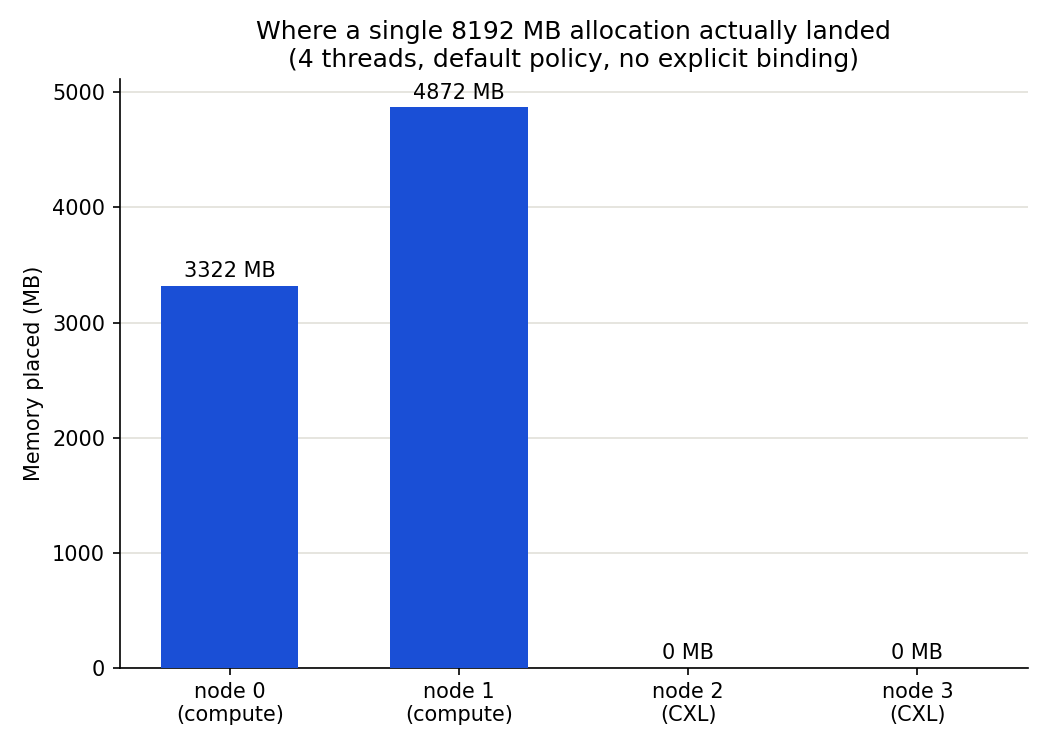
\includegraphics[width=0.6\textwidth,keepaspectratio]{idea1_scatter.png}
  \caption{Where a single 8\,GB allocation landed under the default policy: 4 threads, no explicit binding.}
  \label{fig:scatter}
\end{figure}}{}

\paragraph{Idea 3: cost of data ending up on CXL.}
Testing genuine, natural memory overflow onto CXL would require pushing a node's real free memory low enough to trigger the kernel's own fallback behavior. On this shared machine, node~0 currently has only about 87\,GB free, meaning forcing real overflow would mean consuming most of the currently available memory, which is not necessarily a good idea on a shared machine. The NUMA locality result earlier in this document already answers the same underlying question safely: local memory achieved 14.9\,GB/s, while CXL memory achieved 10.7\,GB/s under the same workload (Section~3).

%------------------------------------------------------------
\section{Designing a CXL-Aware Allocator}

Before implementing anything, it is worth laying out the plan and why, since the evidence gathered across this whole project already points toward some concrete design choices.

\paragraph{The starting problem.}
NUMAlloc's entire design assumes every node has both CPUs and memory: bind a thread to a node, bind memory to that same node. This machine's CXL nodes have memory and no CPUs at all, so there is no thread to bind there. NUMAlloc's model does not actually extend to this case; to NUMAlloc, CXL is just another remote node, and the locality test earlier in this document shows that is a real, meaningfully worse remote node (about 28\% less bandwidth than same-tier cross-socket DDR, about 40\% less than local). So rather than trying to make a CXL-aware allocator bind to CXL the same way NUMAlloc binds to a regular node, we should probably decide which allocations might belong on fast local memory, and which could go on the larger but slower CXL tier.

A few things measured in this document seem worth taking into account, rather than guessing at the design from scratch.

\paragraph{First: TLB reduction is the real advantage.}
Most importantly, NUMAlloc's real advantage turns out to be TLB reduction, not locality, which is exactly the mechanism a CXL tier needs to inherit. Across every condition tested in this document (the main results, AutoNUMA disabled, and the cpunodebind/membind test), NUMAlloc's runtime wins traced back more consistently to fewer TLB misses via hugepage sharing than to fewer remote accesses. Remote-access avoidance looked far less reliable as a source of advantage: it reversed entirely for dedup, and got worse rather than better for streamcluster, depending on the memory policy. TLB reduction, by contrast, held up across every condition tested. That is the one piece of NUMAlloc's design most worth carrying over deliberately into the CXL tier, though this is based on a handful of experiments, not something I would treat as fully settled yet.

\paragraph{Second: more placement freedom does not automatically help.}
Giving the allocator more freedom in where to place memory does not automatically help, which matters directly for how a CXL tier should be designed. The cpunodebind/membind test showed that letting the OS choose between two allowed nodes, rather than forcing one, made NUMAlloc's remote-access count worse across the board, and made streamcluster specifically go from tied to a clear loss. Letting an allocator pick from more than one place is not obviously an improvement; it needs to be tested directly once a real CXL tier exists, not assumed.

\paragraph{Third: placement probably should not be reactive.}
The AutoNUMA experiment suggested that observe-then-migrate mechanisms carry real, measurable overhead that needs sustained runtime to pay off, and a CXL migration crosses a slower link than a same-tier NUMA one, so an automatic hot/cold migration approach might cost more here, not less. A reasonable starting point is a simple, explicit rule decided once at allocation time (e.g., a size threshold, or an explicit hint from the caller), rather than a background migration system, at least to start with.

\paragraph{Origin-aware deallocation.}
On origin-aware deallocation specifically, it is not yet clear whether it is worth extending to a CXL tier the same way: freed CXL objects could return to a CXL-tier freelist matching their origin, the same principle NUMAlloc applies locally. Whether that is actually necessary for a two-tier (rather than multi-node) system is still an open question.

\paragraph{First version.}
Concretely, the first version should aim for:
\begin{itemize}[nosep]
  \item runtime detection of which nodes actually have CPUs (rather than a hardcoded node count, unlike NUMAlloc; see Idea~2);
  \item a size threshold with an explicit hint API for override;
  \item once that is working, hugepage sharing for the CXL tier.
\end{itemize}
Once built, the plan is to validate it the same way Figure~4 was replicated here (runtime, remote accesses, and TLB misses), compared against NUMAlloc and the other allocators already tested throughout this document.

%------------------------------------------------------------
\section{Next Step: Access-Pattern-Aware Placement}

Worth reading into before settling on a final placement policy: rather than deciding local vs.\ CXL purely from allocation size, known access patterns (sequential vs.\ random) could matter too. If an access pattern is predictable enough to prefetch, some of CXL's extra latency might be hidden that way, making CXL a reasonable place for data that would otherwise seem too latency-sensitive for it.

A recent paper from the lab on handling latency in tiered memory~\cite{tolerate} looks like a good starting point. The next step is to read it, understand how it uses prefetching to hide CXL latency, and figure out whether and how that idea should factor into the placement policy here, alongside, or possibly instead of, the size-threshold approach discussed above.

\begin{thebibliography}{9}
\bibitem{numalloc} H.~Yang, X.~Zhao, J.~Zhou, W.~Wang, S.~Kundu, B.~Wu, H.~Guan and T.~Liu. NUMAlloc: A Faster NUMA Memory Allocator. \emph{ACM SIGPLAN International Symposium on Memory Management (ISMM)}, 2023. \url{https://doi.org/10.1145/3591195.3595276}
\bibitem{glibc234} C.~O'Donell. The GNU C Library version 2.34 is now available. libc-announce, August 2021. \url{https://sourceware.org/pipermail/libc-announce/2021/000032.html}
\bibitem{tolerate} M.~\"Unal, V.~Gupta, Y.~Pan, Y.~Ren and S.~Kashyap. Tolerate It if You Cannot Reduce It: Handling Latency in Tiered Memory. \emph{Workshop on Hot Topics in Operating Systems (HotOS)}, 2025. \url{https://doi.org/10.1145/3713082.3730376}
\bibitem{repo} A.~Bekkar. cxl-alloc-benchmarks: scripts, fixes and results of this evaluation. \url{https://github.com/Zeleph25/cxl-alloc-benchmarks}
\end{thebibliography}

\end{document}